\setlength{\parindent}{0em} 

%**********************************************************************************
% Kapitel Anforderungsmatrix
%**********************************************************************************
\chapter{Anforderungsmatrix}\label{Anforderungsmatrix}

%**********************************************************************************
% Kapitel Allgemeines
%**********************************************************************************
\section{Allgemeines}
Die Analyse der in Kapitel \ref{Übersicht_Literatur} beschriebenen Richtlinien ergab insgesamt 417 Anforderungen an IT-Sicherheit (269 organisatorische, 148 technische), die von Banken in Österreich umzusetzen sind. 
Diese Anforderungen wurden zur besseren Übersicht und zur weiteren Bearbeitung in eine Anforderungsmatrix übernommen. In diesem Kapitel wird der Grundaufbau der Anforderungsmatrix und der Erstellungsprozess genauer beschrieben. Im Anschluss daran wird die Anforderungsmatrix ausgewertet. 

%**********************************************************************************
% Kapitel Aufbau
%**********************************************************************************
\section{Aufbau}
Die Anforderungsmatrix gliedert sich in die 5 Bereichen \glqq{}Allgemeines\grqq{}, \glqq{}Institution\grqq{}, \glqq{}Relevanz\grqq{}, \glqq{}Risiko\grqq{} und \glqq{}Umsetzbarkeit\grqq{}.
Diese 5 Bereiche werden innerhalb von 23 Sub-Bereichen weiter untergliedert. Jede technische IT-Sicherheitsanforderung wird auf Basis der Bereiche und Sub-Bereiche näher definiert. 
\bigbreak
In folgendem Kapitel werden die Bereiche und die Sub-Bereiche der Anforderungsmatrix beschrieben. 

\subsubsection{Allgemeines}
Dieser Bereich bietet allgemeine Informationen über die Anforderungen und beinhaltet folgende Elemente:
\bigbreak
\begin{itemize}
    \item \textbf{\#} \\
    Diese Spalte stellt die fortlaufende Nummerierung der Anforderungen dar.
    \item \textbf{Kategorie}\\
    Jede Anforderungen ist einer Kategorien zugewiesen, welche die Anforderung bestmöglich beschreibt. Die Kategorien ermöglichen die Aufteilung der Anforderung in unterschiedliche Themengebiete, die sich im Laufe der Ausarbeitung der Anforderungsmatrix herauskristallisiert haben. 
    \item \textbf{Titel der Anforderung}\\
    Der \glqq{}Titel der Anforderung\grqq{} liefert Informationen zum Kapitel, unter dem die Anforderung in der jeweiligen Richtlinie angeführt ist. Der Titel dient gleichermaßen als umzusetzendes Themengebiet als auch als nähere Beschreibung der Kategorie.
    \item \textbf{Definition}\\
    Der Bereich \glqq{}Definition\grqq{} definiert die tatsächlich umzusetzende Anforderung. 
    \item \textbf{Beschreibung}\\
    In diesem Bereich wird die umzusetzende Anforderung, nach dem Schema \glqq{}Wer\grqq{} hat \glqq{}Wann\grqq{}, \glqq{}Was\grqq{} zu tun um die Anforderung zu erfüllen, beschrieben.
    \item \textbf{Referenz}\\
    Der Bereich \glqq{}Referenz\grqq{} stellt eine Verbindung zum Dokument, in dem die Anforderung enthalten ist.
\end{itemize}
\bigbreak
\subsubsection{Institution}
Dieser Bereich liefert Informationen über die jeweilige Richtlinie aus der die Anforderung abgeleitet wurde. 
\begin{itemize}
    \item \textbf{Institution}\\
    Dieses Feld definiert die Aufsichtsbehörde, welche die Richtlinie veröffentlicht hat.
    \item \textbf{Typ}\\
    Der \glqq{}Typ\grqq{} gibt genauere Informationen über die Ausprägung der jeweiligen Richtlinie.
    \item \textbf{Dokument}\\
    Dieses Feld bietet eine Referenz auf die jeweilige Richtlinie.
    \item \textbf{Version / Fassung}\\
    Die Version / Fassung bietet weitere Informationen zur analysierten Ausgabe der Richtlinie.
\end{itemize}
\bigbreak
\subsubsection{Anforderung}
Dieser Bereich liefert Informationen darüber, ob es sich bei der Anforderung um eine EU-weite Regelung handelt, die Anforderung speziell für Österreich gilt oder für andere Länder relevant ist. Aufgrund der wirtschaftlichen Nähe zwischen Österreich und Deutschland, können sich österreichische Prüfungsorgane auch an deutschen Richtlinien orientieren.  
\begin{itemize}
    \item \textbf{EU}\\
    Gibt an, dass es sich bei der Anforderung um eine EU-weite Richtlinie handelt.
    \item \textbf{AT}\\
    Gibt an, dass die Anforderung nur in Österreich Gültigkeit besitzt. 
    \item \textbf{Andere}\\
    Definiert das Land für das die jeweilige Anforderung gilt, falls die Anforderung nicht EU-weit gültig oder ausschließlich für Österreich gültig ist.
\end{itemize}
\bigbreak
\subsubsection{Risiko}
Der Bereich \glqq{}Risiko\grqq{} beschreibt den der Anforderung zugrunde liegenden Risikofaktor. 
\begin{itemize}
    \item \textbf{Risikofaktor}\\
    Der \glqq{}Risikofaktor\grqq{} unterteilt das durch die Anforderung adressierte Risiko in die Bereiche \glqq{}Technisch\grqq{}, \glqq{}Organisatorisch\grqq{}, \glqq{}Menschlich\grqq{} und \glqq{}Rechtlich\grqq{}. Die unterschiedlichen Bereiche werden in Kapitel \ref{Auswertung_der_Anforderungsmatrix_Vorgehen} genauer beschrieben.
\end{itemize}
\bigbreak
\subsubsection{Umsetzbarkeit} \label{umsetzbarkeit_maßnahme}
Im Zuge der Umsetzbarkeit wird analysiert, wie und durch welche Maßnahme die Anforderung umgesetzt werden kann. Auf Basis der Maßnahmen wird auf Best-Practice-Ansätze geschlossen. 
\begin{itemize}
    \item \textbf{Technisch}\\
    Die Anforderung kann mit Hilfe von technischen Mitteln umgesetzt werden. 
    \item \textbf{Beschreibung}\\
    Beschreibung der technischen Umsetzbarkeit.
    \item \textbf{Organisatorisch}\\
    Die Anforderung kann organisatorisch umgesetzt werden.
    \item \textbf{Beschreibung}\\
    Beschreibung der organisatorischen Umsetzbarkeit.
    \item \textbf{Abgedeckt durch Maßnahme x}\\
    Dieser Sub-Bereich beschreibt die konkreten Maßnahmen für die Umsetzung. An Hand dieser Maßnahmen werden im Zuge der Ausarbeitung Best-Practice-Ansätze definiert.
\end{itemize}
\bigbreak

%**********************************************************************************
% Kapitel Erstellung
%**********************************************************************************
\section{Erstellung}\label{Auswertung_der_Anforderungsmatrix_Vorgehen}
Im ersten Schritt wurde der Inhalt der Richtlinien aus Kapitel \ref{Übersicht_Literatur} analysiert und die darin enthaltenen Anforderungen in den Bereichen \glqq{}Allgemeines\grqq{}, \glqq{}Institution\grqq{} und \glqq{}Anforderung\grqq{} niedergeschrieben. Im Zuge der Ausarbeitung wurden sämtliche evaluierten Anforderungen in die Matrix übernommen und der Fokus nicht nur auf technisch umsetzbare Anforderungen gelegt. Dies hat den Grund, dass auch auf den ersten Blick vermeintlich organisatorisch zu lösende Anforderungen unter Umständen technisch umgesetzt werden können und vice versa.
\bigbreak
Im zweiten Schritt wurden die Anforderungen auf Basis ihres Inhalts gruppiert und in weiterer Folge entsprechend nach Themengebiet kategorisiert. Für die Kategorisierung, zu finden im Bereich \glqq{}Allgemein\grqq{} - \glqq{}Kategorie\grqq{ }, wurden passende Themengebiete gewählt, welche die jeweiligen Anforderungen bestmöglich beschreiben.
\bigbreak
Im dritten Schritt wurde festgelegt, ob die jeweilige Anforderung für Unternehmen in der Europäischen Union, Österreich oder anderen Ländern gültig ist.
\bigbreak
Im vierten Schritt wurde den Anforderungen jeweils ein Risikofaktor zugewiesen. 
Im Zuge der Ausarbeitung haben sich folgende Risikofaktoren als passend erwiesen:

\begin{itemize}
    \item Technischer Risikofaktor
    \item Organisatorischer Risikofaktor
    \item Menschlicher Risikofaktor
    \item Rechtlicher Risikofaktor
\end{itemize}

%**********************************************************************************

\subsubsection{Technischer Risikofaktor}
Dieser Risikofaktor bedeutet, dass die Anforderung auf den Schutz von Vertraulichkeit, Integrität oder Verfügbarkeit des zu schützenden Assets ausgelegt ist. Ein Beispiel dafür ist die Anforderung, dass Organisationen sich laufend über Bedrohungen und Schwachstellen des Informationsverbundes zu informieren, deren Relevanz zu prüfen, diese zu Bewertung und entsprechend Maßnahmen zu ergreifen haben. Ein nicht einhalten dieser Anforderung könnte in einem Angriff mittels Malware über eine Schwachstelle im System oder etwa einem Denial-of-Service Angriff resultieren. Beide Angriffe würden die Vertraulichkeit, Integrität oder Verfügbarkeit der Systeme und der darin enthaltenen Daten gefährden. 

\subsubsection{Organisatorischer Risikofaktor}
Dieser Risikofaktor adressiert Anforderungen, die auf den Erhalt von Kontrolle, Kommunikation, Information oder Nachvollziehbarkeit von Prozessen und Abläufen innerhalb des Unternehmens ausgelegt sind. Ein Beispiel bietet die Anforderung an Unternehmen, die Rolle eines Informationssicherheitsbeauftragten zu etablieren. Wird dieser Anforderung nicht nachgekommen können diverse sicherheitsrelevante Prozesse nicht eingehalten und relevante Informationen gegebenenfalls nicht kommuniziert werden.  

\subsubsection{Menschlicher Risikofaktor}
Anforderungen mit diesem Risikofaktor dienen dem Schutz von Mitarbeiter*innen und Kund*innen des Unternehmens. Ein Beispiel ist die Anforderung an Unternehmen, ein kontinuierliches und angemessenes Sensibilisierung- und Schulungsprogramm für Informationssicherheit festzulegen und den Erfolg der Maßnahmen regelmäßig zu überprüfen. Wird diese Anforderung nicht erfüllt fehlt den Mitarbeitern des Unternehmens Awareness im Bereich IT-Sicherheit. Eine mögliche Auswirkung könnte ein erfolgreicher Phishing-Angriff per Email sein. In diesem Fall könnte auch der Mitarbeiter zur Verantwortung gezogen werden. 

\subsubsection{Rechtlicher Risikofaktor}
Anforderungen mit diesem Risikofaktor schützen Unternehmen vor Imageschäden, Strafgebühren, Strafverfolgung oder monetären Schäden. Ein Beispiel hierfür ist die Anforderung, dass Unternehmen sicherzustellen haben, dass Tests und Überprüfungen zur Informationssicherheit von unabhängigen Prüfern mit ausreichenden Kenntnissen, Fähigkeiten und Fachwissen durchgeführt werden. Eine Auswirkung der Nichteinhaltung könnte eine Strafverfolgung aufgrund eines Angriffs sein, bei dem Kundendaten entwendet wurden. Kann das Unternehmen nicht nachweisen, dass der implementierte Schutz zur Informationssicherheit den geforderten Standards entspricht, könnte das Unternehmen hier haftbar gemacht werden.
\bigbreak
Im letzten Schritt wurde Bezug auf die Umsetzbarkeit der einzelnen Anforderungen genommen. Hierbei wurde unterschieden, ob sich die Anforderung technisch und / oder organisatorisch umsetzen lässt. Im Zuge dessen wurde analysiert, mit welchen Maßnahmen sich die technischen Anforderung umsetzen lassen. Hierfür wurden pro Anforderung bis zu vier Maßnahmen definiert. Aus diesen Maßnahmen werden in weiterer Folge Best-Practice-Ansätze abgeleitet. 

%**********************************************************************************
% Kapitel Auswertung und Erkenntnisgewinn
%**********************************************************************************
\section{Auswertung und Erkenntnisgewinn}
Im Zuge der Ausarbeitung der in Tabelle \ref{table:uebersicht_verwendete_literatur} ausgewählten Richtlinien konnten 417 IT-Sicherheitsanforderungen an eine Bank in Österreich abgeleitet werden. Diese Anforderungen unterteilen sich in 148 Anforderungen die technisch umzusetzen sind und 269 Anforderungen die organisatorisch umzusetzen sind, wie in Tabelle \ref{table:anforderungen_vergleich} ersichtlich. Interessant ist die Erkenntnis, dass zwei Drittel der Anforderungen an IT-Sicherheit für Banken in Österreich keinen technischen Hintergrund besitzen.
\bigbreak
\begin{table}[H]
    \centering
    \caption{Übersicht technischer und organisatorischer Anforderungen.} 
    \begin{tabular}{lll}
        \hline
        Anforderung & Anzahl & Prozentanteil \\
        \hline\hline
        Organisatorisch & 269 & 64.5\%\\
        Technisch & 148 & 32.5\%\\
        \hline
        Gesamt & 417 & 100 \%
    \end{tabular}
    \label{table:anforderungen_vergleich}
\end{table}
\bigbreak
Im Zuge der Ausarbeitung der Anforderungsmatrix, konnten die Richtlinien folgenden Kategorien zugeordnet werden:
\begin{itemize}
    \item Auslagerung und Fremdbezug IT-Dienstleistungen
    \item Business-Continuity Management
    \item Identity- und Access-Management
    \item Informationsrisikomanagement
    \item Informationssicherheitsmanagement
    \item IT-Betrieb
    \item IT-Projekte und Anwendungsentwicklung
    \item IT-Strategie
    \item Management Zahlungsdienstleister
    \item Management Zahlungsdienstnutzer
    \item Operative Informationssicherheit
\end{itemize}
\bigbreak
Die Kategorie \glqq{}Auslagerung und Fremdbezug IT-Dienstleistungen\grqq{} vereint alle Anforderungen die sich auf die Auslagerung von Funktionen, Tätigkeiten und Systemen beziehen. Des Weiteren wird in diesen Anforderungen festgelegt, wie mit Dienstleistungen umzugehen sind, die von Dritten bezogen werden. Ein Beispiel für eine Anforderung aus dieser Kategorie ist, dass für jeglichen Fremdbezug von IT-Dienstleistungen vorab eine Risikobewertung durchzuführen ist und die Organisation diese Bewertung laufend zu überwachen und aktuell zu halten hat. Im Bereich \glqq{}Business-Continuity Management\grqq{} sind Anforderungen enthalten, die sich auf den stabilen Betrieb des Unternehmens beziehen. Ein Beispiel hierfür ist die Anforderung, dass für den Fall einer Störung oder einem Notfall wirksame Maßnahmen zur internen und externen Krisenkommunikation zu definieren sind.
\bigbreak
Die Kategorie \glqq{}Identity- und Access-Management\grqq{} vereint Anforderungen die sich auf das Management von Benutzeraccounts, die Vergabe von Berechtigungen und den Zugriff auf IT-Ressourcen beziehen. So besteht etwa die Anforderung, dass ein Prozess zur Regelung von Berechtigungsvergaben auf IT-Ressourcen zu definieren ist. Dies schützt Unternehmen vor einer missbräuchlichen Verwendung oder einer unautorisierten Manipulation von Daten und IT-Systemen. In der Kategorie \glqq{}Informationsrisikomanagement\grqq{} sind Anforderungen rund um die Themen Risikoanalyse, Schutzbedarfsanalyse und Risikobewertung definiert. So haben Unternehmen beispielsweise der Forderung nachzukommen, dass IT-Assets, Geschäftsfunktionen und Unterstützungsprozesse in Hinblick auf deren Kritikalität entsprechend einzustufen sind. 
\bigbreak
Die Richtlinien in der Kategorie \glqq{}Informationssicherheitsmanagement\grqq{} beschäftigen sich mit der Compliance und Governance von Unternehmen. So ist die Geschäftsleitung eines Unternehmens etwa verpflichtet die Funktion eines Informationssicherheitsbeauftragten zu etablieren und diesen zu stellen. Unter die Kategorie \glqq{}IT-Betrieb\grqq{} fallen Anforderungen die sich um das Management, die Verfügbarkeit und den physischen Schutz von IT-Ressourcen drehen. Ein Unternehmen ist verpflichtet Konzepte zur Hochverfügbarkeit zu implementieren, diese anzuwenden und entsprechend zu überprüfen. 
\bigbreak
Der Bereich \glqq{}IT-Projekte und Anwendungsentwicklung\grqq{} umfasst Anforderungen die sich mit der Steuerung von Projekten und der Entwicklung von eigenen Anwendungen beschäftigen. Ein Beispiel für eine Anforderung aus dieser Kategorie ist, dass ein Unternehmen für Projekte ausreichende personelle Ressourcen zur Verfügung zu stellen hat. Die Kategorie \glqq{}IT-Strategie\grqq{} beinhaltet Anforderungen an die strategische Ausrichtung eines Unternehmens, die Aus- und Weiterbildung von Mitarbeitern und der Festlegung von Zuständigkeiten. So hat die Geschäftsleitung eines Unternehmens eine IT-Strategie zu erstellen die im Einklang mit Art, Umfang und Komplexität der Geschäftstätigkeit steht. 
\bigbreak
Die beiden Kategorien \glqq{}Management Zahlungsdienstleister\grqq{} und \glqq{}Management Zahlungsdienstnutzer\grqq{} behandeln Anforderungen zum Schutz von Kunden und Kundentransaktionen. So ist ein Unternehmen beispielsweise verpflichtet seine Kunden über mögliche neue Gefahren, Schwachstellen oder Änderungen in IT-Systemen zu informieren. In der letzten Kategorie \glqq{}Operative Informationssicherheit\grqq{} sind Anforderungen zusammengefasst, die sich mit dem Thema IT-Sicherheit und der technischen Implementierung von IT-Sicherheitsmaßnahmen beschäftigen. So ist ein Unternehmen beispielsweise verpflichtet, Daten bei der Speicherung und der Übertragung gemäß definiertem Schutzbedarf zu verschlüsseln. 
\bigbreak
Tabelle \ref{table:kategorien_gesamt} zeigt die Aufteilung der Anforderungen auf die unterschiedlichen Kategorien. 

\begin{table}[H]
    \centering
    \caption{Kategorien der Anforderungsmatrix und die Anzahl der zugeordneten Anforderungen.} 
    \begin{tabular}{ll}
        \hline
        Kategorie & Anzahl\\
        \hline\hline
        Auslagerung und Fremdbezug IT-Dienstleistungen & 53\\
        Business-Continuity Management & 14\\
        Identity- und Access-Management & 31\\
        Informationsrisikomanagement & 49\\
        Informationssicherheitsmanagement & 35\\
        IT-Betrieb & 47\\
        IT-Projekte und Anwendungsentwicklung & 40\\
        IT-Strategie & 38\\
        Management Zahlungsdienstleister & 12\\
        Management Zahlungsdienstnutzer & 46\\
        Operative Informationssicherheit & 52\\
    \end{tabular}
    \label{table:kategorien_gesamt}
\end{table}


Abbildung \ref{fig:kategorien_allg_aufteilung} zeigt die prozentuale Verteilung aller Anforderungen auf die unterschiedlichen Kategorien. Es sind keine Ausreißer zu erkennen, mit Ausnahme von \glqq{}Management Zahlungsdienstnutzer\grqq{} und \glqq{}Business-Continuity Management\grqq{} verteilen sich die Anforderungen gleich auf die unterschiedlichen Kategorien. 
\bigbreak
\begin{figure}[H]
    \centering
  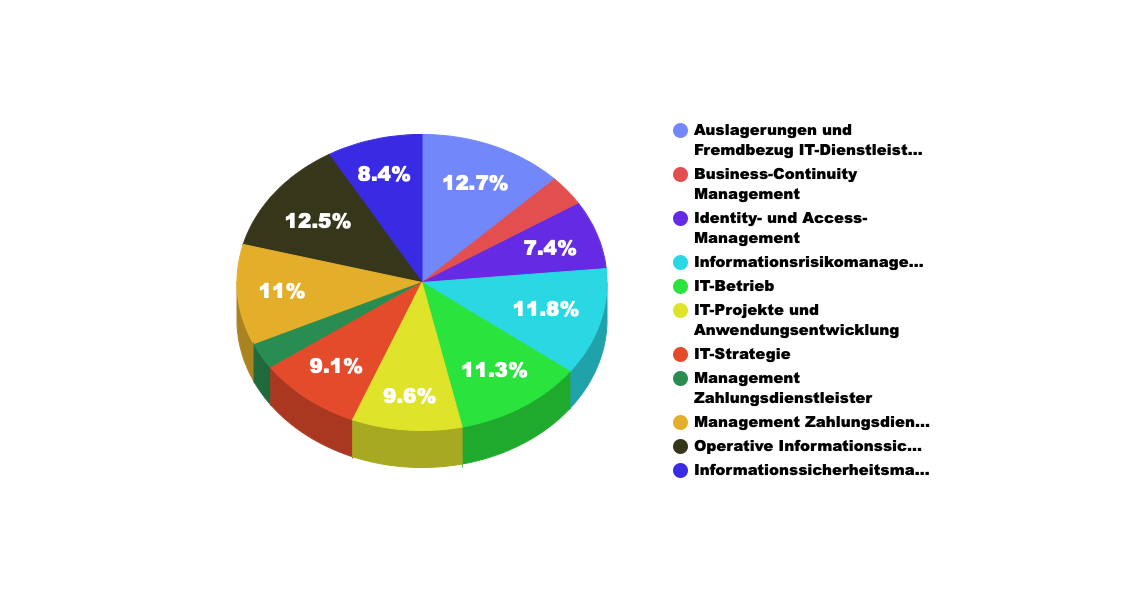
\includegraphics[width=\linewidth]{images/uploads/a_figure_02.png}
  \caption{Visuelle Darstellung der Aufteilung aller Anforderungen auf die definierten Kategorien. Quelle: Eigene Darstellung, 2022}
  \label{fig:kategorien_allg_aufteilung}
\end{figure}

%**********************************************************************************

\bigbreak
Betrachtet man in weiterer Folge nur jene Anforderungen die technisch umzusetzen sind, ergibt sich die in Tabelle \ref{table:kategorien_technisch} dargestellte Aufteilung. Es ist zu erkennen, dass die technisch umzusetzenden Anforderungen vorwiegend in den Kategorien \glqq{}Identity- und Access-Management\grqq{}, \glqq{}IT-Betrieb\grqq{} und vor allem in der Kategorie \glqq{}Operative Informationssicherheit\grqq{} zu finden sind. Abbildung \ref{fig:kategorien_technisch_aufteilung} zeigt die prozentuale Verteilung der technischen Anforderungen auf die unterschiedlichen Kategorien. 
\bigbreak
\begin{table}[H]
    \centering
    \caption{Zeigt die Kategorien der Anforderungsmatrix und die Anzahl der zugeordneten, technischen Anforderungen.} 
    \begin{tabular}{ll}
        \hline
        Kategorie & Anzahl\\
        \hline\hline
        Auslagerung und Fremdbezug IT-Dienstleistungen & 1\\
        Business-Continuity Management & 1\\
        Identity- und Access-Management & 30\\
        Informationsrisikomanagement & 7\\
        Informationssicherheitsmanagement & 11\\
        IT-Betrieb & 31\\
        IT-Projekte und Anwendungsentwicklung & 2\\
        IT-Strategie & 1\\
        Management Zahlungsdienstleister & 0\\
        Management Zahlungsdienstnutzer & 18\\
        Operative Informationssicherheit & 46\\
    \end{tabular}
    \label{table:kategorien_technisch}
\end{table}
\begin{figure}[H]
    \centering
  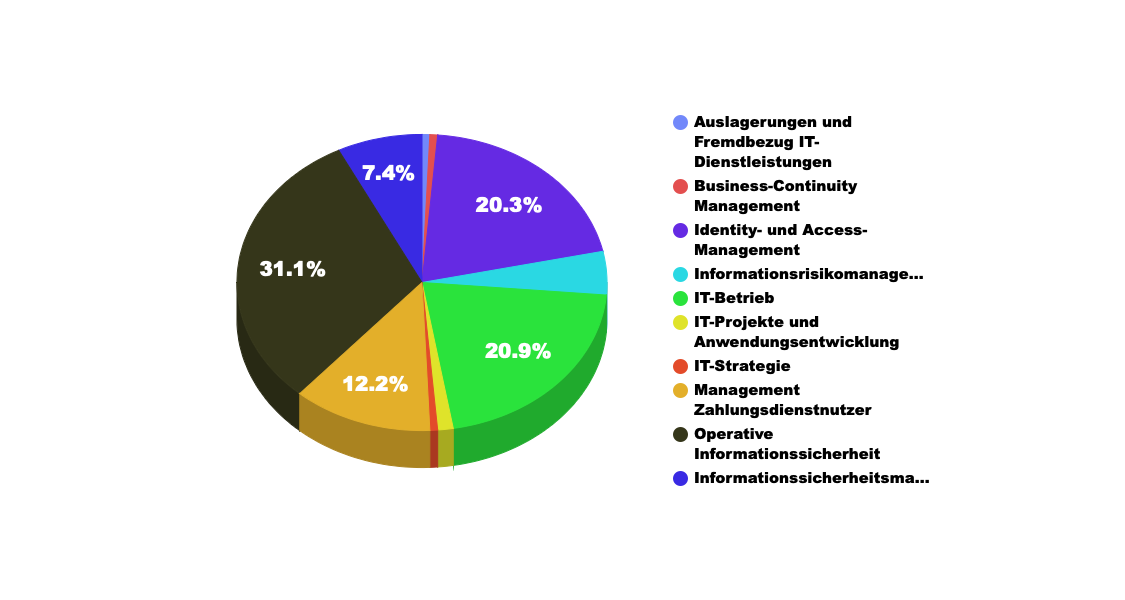
\includegraphics[width=\linewidth]{images/uploads/a_figure_04.png}
  \caption{Visuelle Darstellung der Aufteilung von technischen Anforderungen auf die definierten Kategorien. Quelle: Eigene Darstellung, 2022}
  \label{fig:kategorien_technisch_aufteilung}
\end{figure}
\bigbreak

Zur besseren Veranschaulichung wurden die organisatorisch und technisch umzusetzenden Anforderungen in Tabelle \ref{table:kategorien_vergleich_gesamt} direkt gegenübergestellt. Es ist zu erkennen, dass es nur eine Anforderungen aus dem Bereich \glqq{}Auslagerung und Fremdbezug IT-Dienstleistungen\grqq{} gibt, die sich technisch umsetzen lässt. Es handelt sich dabei um die Anforderung, dass Informationen die mit Drittanbietern ausgetauscht werden verschlüsselt übertragen werden müssen. Alle anderen Anforderungen liegen in der Durchführung bei dem jeweiligen Auslagerungspartner. Die technischen Anforderungen bestehen somit auf Seiten des Dritten. Auch im Bereich \glqq{}Business-Continuity Management\grqq{} besteht nur eine technische Anforderung. Es handelt sich dabei um die Notwendigkeit für eine redundante Auslegung von kritischen IT-Komponenten.
\bigbreak
Im Gegensatz zu den eben genannten Kategorien, sind 30 von 31 Anforderungen aus dem Bereich \glqq{}Identity- und Access-Management\grqq{} technischer Natur. Bei einer organisatorischen Anforderungen handelt es sich um die Notwendigkeit die implementierten, technischen Zugangskontrollen zu überwachen. Interessant ist, dass nur 5\% der Anforderungen aus dem Bereich \glqq{}IT-Projekte und Anwendungsentwicklung\grqq{} technisch erfüllt werden können. Es geht dabei um die Vorgabe, dass eigens erstellte Anwendungen auf mögliche Abweichungen vom Regelbetrieb zu überwachen und die Integrität der Anwendung, insbesondere des Quellcodes, angemessen sicherzustellen ist. 
\bigbreak
Ein weiterer Ausreißer findet sich im Bereich \glqq{}IT-Strategie\grqq{}. Nur eine Anforderung kann technisch umgesetzt werden. Es geht dabei um die Notwendigkeit, dass die Geschäftsleitung imstande sein muss Aussagen zu selbst entwickelten oder selbst betriebenen IT-Systemen treffen zu können. Auch wenn für die Umsetzung der Anforderung nur Informationen nötig sind, kann die Effizienz durch ein Verwaltungssystem, wie beispielsweise einer Content-Management-Database (CMDB) gesteigert werden. Im Bereich \glqq{}Operative Informationssicherheit\grqq{} bestehen 6 Anforderungen die organisatorisch umzusetzen sind. Diese Anforderungen wurden nicht als \glqq{}Technische Anforderung\grqq{} deklariert, da die Umsetzung vorrangig organisatorisch zu definieren ist. Ein Beispiel hierfür ist die Vorgabe, dass ein Zahlungsdienstkunde eine Warnung erhält, bevor eine dauerhafte Sperre seines Accounts in Kraft tritt.
\bigbreak

\begin{table}[H]
    \centering
    \tiny
    \caption{Zeigt alle Kategorien und die Anzahl der zugeordneten Anforderungen.} 
    \begin{tabular}{llll}
        \centering
        Kategorie & Gesamt & Organisatorisch & Technisch\\
        \hline\hline
        Auslagerung und Fremdbezug IT-Dienstleistungen & 53 & 52 & 1\\
        Business-Continuity Management & 14 & 13 & 1\\
        Identity- und Access-Management & 31 & 1 & 30\\
        Informationsrisikomanagement & 49 & 42 & 7\\
        Informationssicherheitsmanagement & 35 & 14 & 11\\
        IT-Betrieb & 47 & 16 & 31\\
        IT-Projekte und Anwendungsentwicklung & 40 & 38 & 2\\
        IT-Strategie & 38 & 37 & 1\\
        Management Zahlungsdienstleister & 12 & 12 & 0\\
        Management Zahlungsdienstnutzer & 46 & 28 & 18\\
        Operative Informationssicherheit & 52 & 6 & 46\\
    \end{tabular}
    \label{table:kategorien_vergleich_gesamt}
\end{table}
\bigbreak
%**********************************************************************************

Im Zuge der Auswertung der Anforderungsmatrix wurden auch die Risikofaktoren näher betrachtet. Abbildung \ref{fig:risiko_allg_aufteilung} zeigt die Verteilung der Risikofaktoren bezogen auf die abgeleiteten Anforderungen. Es ist zu erkennen, dass sich je ein Drittel der Risiken auf die beiden Bereiche \glqq{}Technisch\grqq{} und \glqq{}Organisatorisch\grqq{} verteilen. Daraus lässt sich ableiten, dass zwei Drittel der Anforderungen auf den Schutz der Infrastruktur und der internen Abläufe und Prozesse des Unternehmens ausgelegt sind. 
\begin{figure}[H]
    \centering
  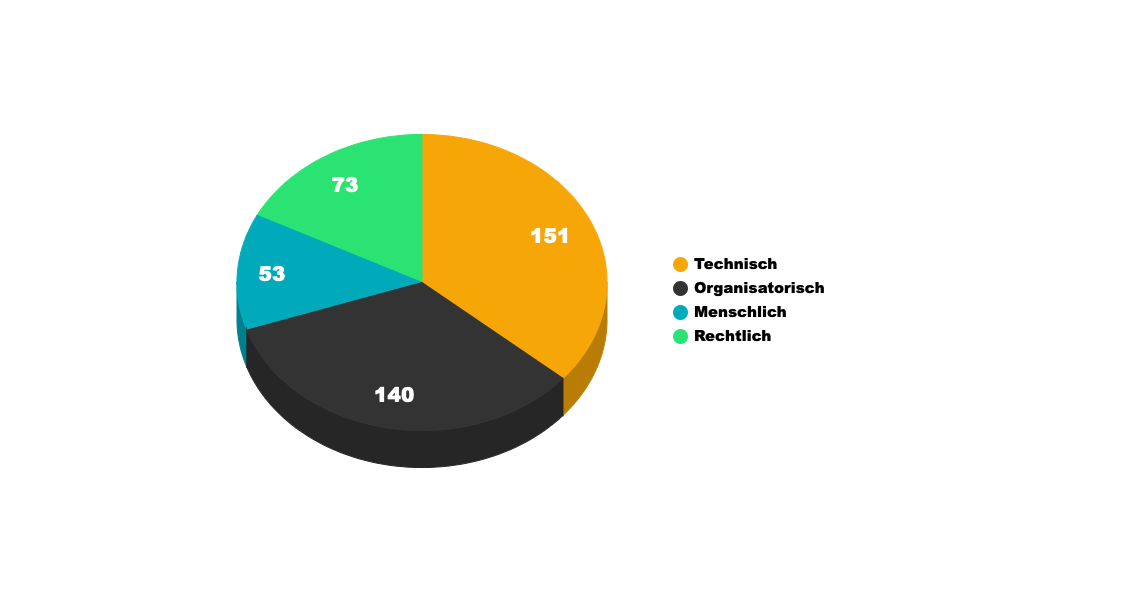
\includegraphics[width=\linewidth]{images/uploads/a_figure_03.png}
  \caption{Visuelle Darstellung der Aufteilung der Risikofaktoren aller Anforderungen. Quelle: Eigene Darstellung, 2022}
  \label{fig:risiko_allg_aufteilung}
\end{figure}
\bigbreak
Abbildung \ref{fig:risiko_technisch_aufteilung} zeigt die Verteilung der technischen Anforderungen auf die unterschiedlichen Risikofaktoren. 
Wie zu erwarten war, adressieren ein Großteil der Anforderungen den \glqq{}Technischen Risikofaktor\grqq{}. Interessant ist hierbei, dass 23 Anforderungen Bezug auf den \glqq{}Menschlichen Risikofaktor\grqq{} nehmen. Es handelt sich dabei um die Anforderungen aus dem Bereich \glqq{}Identity- und Access-Management\grqq{}. Betrachtet man die technischen Anforderungen die den \glqq{}Rechtlichen Risikofaktor\grqq{} adressieren, handelt es sich dabei um die Anforderungen zum Schutz von Transaktionsüberwachungen im Bereich Onlinebanking. Können betrügerische Zahlungen nicht erkannt oder etwa persönliche Sicherheitsmerkmale von Kunden nicht geschützt werden, kann dies rechtliche Konsequenzen für das Unternehmen mit sich ziehen. Bei den technischen Anforderungen die das \glqq{}Organisatorische Risiko\grqq{} adressieren, handelt es sich großteils um Anforderungen zum Umgang und der Verwaltung von IT-Ressourcen. Eine fehlende Verwaltung oder ein nicht definierter Umgang mit IT-Ressourcen kann zu Problemen beim Ablauf interner Prozesse führen und so die Stabilität des Unternehmens gefährden. Anforderungen mit \glqq{}Technischem Risikofaktor\grqq{} beziehen sich unter anderem auf die Implementierung von IT-Sicherheitsmaßnahmen und den Schutz von IT-Ressourcen und Daten. In Anbetracht der Tatsache, dass hierbei nur Anforderungen betrachtet wurden die technisch umgesetzt werden können, erscheint die Aufteilung legitim. 
\begin{figure}[H]
    \centering
  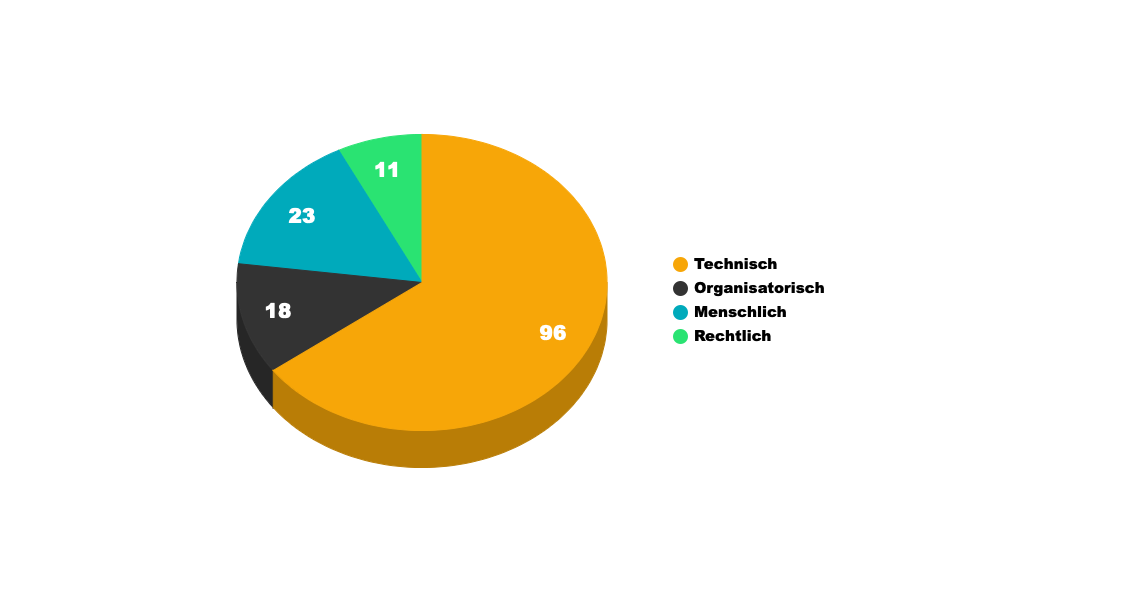
\includegraphics[width=\linewidth]{images/uploads/a_figure_05.png}
  \caption{Visuelle Darstellung der Aufteilung der Risikofaktoren technischer Anforderungen. Quelle: Eigene Darstellung, 2022}
  \label{fig:risiko_technisch_aufteilung}
\end{figure}

%**********************************************************************************
% Karacitel Abgeleitete Maßnahmen
%**********************************************************************************
\section{Abgeleitete Maßnahmen}
\label{kap_anforderungsmatrix_abgleitete_maßnahmen}
Dieses Kapitel gibt eine Übersicht über die aus den Anforderungen abgeleiteten Maßnahmen und zeigt, wie viele Anforderungen die einzelnen Maßnahmen abdecken. Auf Basis dieser Anforderungen wird in weiterer Folge versucht, Best-Practice-Ansätze für die Umsetzung der technischen IT-Sicherheitsvorgaben abzuleiten. Die nötigen Informationen für die Evaluierung der einzelnen Maßnahmen erfolgte auf Basis von Recherchen im Internet und Befragung von Mitarbeitern aus dem Bereichen \glqq{}IT-Security\grqq{} und \glqq{}IT-Infrastruktur\grqq{} einer Bank in Österreich.
\bigbreak
Im Zuge der Erstellung der Anforderungsmatrix wurde im Bereich \glqq{}Umsetzbarkeit\grqq{} definiert, ob die jeweilige Anforderung technisch oder organisatorisch umgesetzt werden kann. Der Bereich \glqq{}Beschreibung\grqq{} bietet eine Zusammenfassung für eine mögliche Umsetzung. Die Bereiche \glqq{}Abgedeckt durch Maßnahme x\grqq{} geben eine Übersicht über mögliche technische Maßnahmen, mit denen die Anforderung umgesetzt werden kann. Für die Evaluierung der möglichen Maßnahmen wurden pro Anforderung folgende Schritte durchgeführt:
\begin{enumerate}
    \item Recherche im Internet mit Hilfe der Informationen aus den Bereichen \glqq{}Kategorie\grqq{}, \glqq{}Titel der Anforderung\grqq{} und \glqq{}Definition\grqq{} der Anforderungsmatrix.
    \item Recherche von möglichen Hardware-/Softwareprodukten zur Adressierung der jeweiligen Anforderung.
    \item Befragung von Mitarbeitern aus den Bereichen \glqq{}IT-Infrastruktur\grqq{}, \glqq{}IT-Technik\grqq{} und \glqq{}Security-Operation-Center\grqq{} einer Bank in Österreich.
\end{enumerate}
\bigbreak
Tabelle \ref{table:maßnahmen_uebersicht_anzahl} zeigt eine Auflistung der abgeleiteten Maßnahmen und die Anzahl der technischen Anforderungen, die mit der jeweiligen Maßnahme umgesetzt werden können. Bei dieser Auswertung ist zu beachten, dass Anforderungen auch mit mehr als einer Maßnahme umgesetzt werden können. Aus diesem Grund variieren die Anzahl der technischen Anforderungen und die Anzahl der in Tabelle \ref{table:maßnahmen_uebersicht_anzahl} dargestellten Maßnahmen.
Interessant ist hierbei, dass sich 15\% der Anforderungen mittels der Adressierung von \glqq{}Identity-Management\grqq{} umsetzen lassen. Das bedeutet, dass Aufsichtsbehörden großen Wert auf den korrekten Umgang mit Berechtigungen und Accounts legen. 10\% der Anforderungen können durch die Betrachtung von \glqq{}Vulnerability-Management\grqq{} und weitere 9\% durch \glqq{}Security Incident und Event Monitoring\grqq{} adressiert werden. Daraus resultiert die Tatsache, dass sich ein Drittel der technischen Anforderungen für IT-Sicherheit an eine Bank in Österreich mit der Implementierung von drei Maßnahmen umsetzen lassen. 


\begin{table}[H]
    \centering
    \caption{Zeigt eine Übersicht über die analysierten Maßnahmen und die Anzahl der adressierten, technischen Anforderungen.} 
    \begin{tabular}{llll}
        Maßnahme & Anzahl adressierter Anforderungen\\
        \hline\hline
        Identity-Management & 32\\
        Vulnerability-Management & 21\\
        Security Incident und Event Monitoring & 20\\
        Kryptografie & 17\\
        Content-Management Database & 15\\
        Multifaktor-Authentifizierung & 15\\
        Patch-Management & 15\\
        Zentrales Log-Management & 13\\
        Netzwerksegmentierung & 11\\
        Monitoring & 10\\
        Single-Sign On & 10\\
        Backup and Restore & 10\\
        Endpoint-Detection and Response & 7\\
        Penetration-Testing & 6\\
        Baselining und Change-Management & 4\\
        Sourcecode Verwaltung & 4\\
        Native-Change Detection & 3\\
        Privileged-Access Management & 3\\
        Hochverfügbarkeit & 3\\
        Firewalls & 2\\
        Network-Access Control & 1
    \end{tabular}
    \label{table:maßnahmen_uebersicht_anzahl}
\end{table}